% Maps
% \pfBigArt{t}{book/img/level1_1}
% \pfBigArt{t}{book/img/level1_2}

% Clearpage is here to keep them at the top of the document
\clearpage

\pfMakeSplashHeader[
  image = images/inside,
  title = Airship Pirates,
  headerHeight = -7cm,
  textBodyHeight = 6cm
]
  
\chapter{Airship Pirates}

\begin{multicols}{2}
\addSidebar % For some reason this is the only spot this can go without being in the wrong place. It adds space before the Overview, though, which is not ideal. TODO
\vspace{-.64in} % There was a spacing anomaly at the top of this, even after adding the 0pt space to the \textarea in the main doc
  \section{Overview}
  This adventure is built as a short hook into a larger story. It serves a few key functions: to give background on how the adventure begins, getting the players right into the action, and to create a thread for the players to pull that will unravel a larger plot. 
  
  This adventure begins on the coast of the Arcadian Ocean in Ravounel, where a fishing town called Daven-Skort has been waylaid by dragon attacks and sustained pirate raids in a most peculiar fashion: by airship! As Pathfinders, the PC's have been called upon as a last resort to protect the town and thwart the pirates.  As they round the last bend of their journey, smoke pillars rise from the town. Mingled in the smoke, a huge airship hovers in the heart of the town, ropes hanging taughtly over the bow. 

  By the end of the first chapter, the PC's will need to make a choice: commandeer the airship and pursue the pirates to their lair, or take the information back to Pathfinder headquarters in Absalom.

  \section{Running The Adventure}
  The following sections detail the setup for the adventure and everything you should know before starting. There are specific headings provided to give you a clear idea of how to steer this adventure. This adventure starts the Pathfinders off as accomplished individuals chosen directly for this mission, and the PC's start at level seven.

  \subsection{Background}
  The PC's were dispatched from Absalom when reports of a dragon attack on the small town of Daven-Skort reached the Pathfinder Society. They have traveled a several day's journey by cart and mule to the sea-side town through Ravounel. Though the journey has been long, it has been thankfully uneventful.
  
  \subsection{The Plot}
  The party arrive at Daven-Skort just as it is repelling its latest siege against an air vessel filled with pirates. The party, being Pathfinders, will be expected to join the fight and assist the town guard to fight back. During the siege, the party will discover that a massive dragon assailed the town in the hours prior the pirates arriving, loosing an inferno on the cliffs and surrounding countryside. 
  
  The town folk were able to contain the fire before it reached the town walls, but the manors on the cliffs have been reduced to cinders. This counts the third time the dragon has attacked Daven-Skort, and every time the pirates have followed to raid and pillage cargo from the galleons of the harbor.

  The captain of the guard will admonish the Pathfinders to commandeer the moored air ship to the pirate's lair and end their raids on the town. As for the dragon, the captain expresses hopes that since they're always seen in tandem, that they must be connected.
  
  \section{Daven-Skort}
  Daven-Skort is a small fishing town founded on the edge of the Arcadian Ocean. Mariner life is prevalent here, as most of the trade and exports from this town to neighboring villages comes from the sea. There is a hint of piracy, and the taverns closest to the port itself are typically rough and rowdy. The architecture of the town is both nautical and practical. 
  
  Among the most striking buildings on the skyline is a one-hundred and seventy-five foot lighthouse that springs from the center of the harbor. The structure itself is built of large stones hewn into curved shapes which start from an elongated base which stands about a quarter of the height at the base. The base of the lighthouse is about four stories tall, and houses the city hall and courts. The lighthouse spire itself has various port holes and lookouts along the winding path to the top, which culminates in a bulbous top, seemingly too large for the thing neck. 

  There are several other notable locations in Daven-Skort, such as the large fish market which takes up the large open area surrounding the lighthouse itself. At one point these weaving alleys of stalls were moved and removed regularly, but as business from the sea is constant in this town, the stalls have become more like shanties and shed their fabric tops for more structurally permanent shacks and shanties.

  Pubs and taverns dot the edge of the large open area surrounding the lighthouse and markets, but the path to the wharf is clear of any buildings as the bounty that drives this town's economy travels unhindered from boats to stalls for sale.

  \subsubsection{History}
  Daven-Skort was a town founded by necessity in Ravounel. Though nowhere near as popular as the Northern port of Vyre, the town sprung up on the Southern side of the same peninsula, on the outcropping of the Dismal Nitch. Some say Daven-Skort was formed by pirates who had used the port as a hideout. Others say privateers with aims of retiring founded the town away from the main road in an effort to quietly live out the rest of their lives in peace.

  Today, Daven-Skort has grown to a population of one thousand people. The thriving port now provides sea fare to cities from Vyre to Kintargo. The road to Daven-Skort is well-work with trade, and the city has sprawled from the sea to the coves and cliff-sides on either side of the town. A few large manors sit atop the cliffs themselves, overlooking the town.

  \subsection{The Gates of Daven-Skort}

  The party has taken a long and winding journey from Absalom through the Shining Kingdoms and Old Cheliax in order to finally reach Ravounel. They've been traveling light in a single cart pulled by two riding horses for many days, and just as they round the last bend to Daven-Skort, one among their number points out the striking sight. A dragon, flying high on the horizon, dives toward the ground and looses a torrent of fire. It then rises in the air and departs toward the ocean.

  \begin{pf-parchment}[\textcolor{title1}{Description}]
    \textcolor{title1}{\textit{The town of Daven-Skort lies ahead the last bend. Two large cliffs jut out on either side of the port town, framing the tall lighthouse that reaches from its center. Pillars of smoke rise from the town, and still burning fires consume the buildings atop the cliffs. Fires rage ahead of the party as well, as the forest trees surrounding the road have caught the blaze.}}
  \end{pf-parchment}

As the party continues down the path toward Daven-Skort, the horses start bucking wildly as the town gate comes into view. The fire in the woods has flushed out a group of three Ankhrav from a hive somewhere in the vicinity, and the creatures burst out of the fire and attack the party.

Note: The wildfire raging in the forest surrounding the fire creates a Flames, Heat, and Smoke natural disaster conditions. If the party ventures too close to the fire itself, have them start taking moderate Heat damage (4d6-6d6) every round they end up within 10 feet of the fire. If they venture into the fire, they take moderate persistent Fire damage, and the Smoke coupled with the Heat causes them to need to hold their breath or suffocate, even within 10 feet, . Throughout the encounter, smoke can cause difficulty seeing the creatures, causing them to be concealed. Wind may carry smoke--and fire--in different directions each turn, as decided by the GM.

After the first round, two more Ankhrav join the fight.

  \textbf{Note: The wildfire raging in the forest surrounding the fire creates a Flames, Heat, and Smoke natural disaster conditions. If the party ventures too close to the fire itself, have them start taking minor Heat damage every round they end up within 10 feet of the fire. \\\\If they venture into the fire, they take moderate persistent Fire damage, and the Smoke coupled with the Heat causes them to need to hold their breath or suffocate. \\\\Throughout the encounter, smoke can cause difficulty seeing the creatures, causing them to be concealed. Wind may carry smoke--and fire--in different directions each turn, as decided by the GM.}

  \begin{creaturebox}{Ankhrav (3)}{5}
    \textit{Monster Core 20}\\
    \textbf{Initiative} Perception +7
  \end{creaturebox}

After the party has taken care of the rogue Ankhravs, they can continue to the open gates of Daven-Skort. Signs of the raiding parties that have ravaged this town over the past few weeks are immediately visible. Burnt-out buildings, destroyed carts and tools, and scorched remains of stock-piled goods are common as the party enters Daven-Skort.

\subsection{The Burning Tree}

A single detachment of guards have formed a bucket brigade to staunch a fresh fire before it leaps onto a nearby building. They pass water from a stone well down the line to a fallen tree engulfed in flame. The guards call out to the party asking for assistance. If the party agrees to help to fight the fire, roll initiative.

Moving too close to the tree itself still has all the environmental effects Flames (4d6-6d6 persistent heat damage), Smoke (obscuring with the Concealed condition), and Heat (minor heat damage a distance, 1d6-2d6).

  \begin{creaturebox}{Flaming Tree}{7}
    \textit{Complex Hazard}\\
    \textbf{Stealth} 24 (expert)\\
    \textbf{Description} The wildfire in the surrounding forest has caused a tree to fall dangerously close to a nearby structure.\\
    \textbf{Disable} DC 23 Survival (trained) to put out the fire with water or dirt. Three consecutive successes are required to disable the hazard.\\
    \textbf{AC} 24; \textbf{Fort} +15, \textbf{Ref} +15\\
    \textbf{HP} 62 (BT 16); \textbf{Immunities} critical hits, object immunities, precision damage\\
    \textbf{Routine} (1 action) The fire grows 5 feet each turn in the direction of the closest combustable structure.\\  
    \begin{pf-reaction}{Crackling Flame}{A creature enters a space within 5 feet of the hazard.}
      The wind blows the wild fire in the direction of the creature scalding them for 2d10+9 fire damage.
    \end{pf-reaction}
  \end{creaturebox}

  \subsection{The Captain of the Guard}

  After the guards and the party put out the fire, one of their number thanks the party for their assistance. If the party identifies themselves as Pathfinders sent to help the situation or simply as able bodies to assist in the crisis, the guard directs them to the captain of the guard in the barracks near the North end of town. The guard might mention the size of the dragon as it unleashed its flaming breath on the countryside. If the party refuses to go to the Captain and wants to make their own way, the guard shrugs and the brigade moves on from the area looking for more fires to fight. 

At this point the whole of Daven-Skort is available for the party to navigate through, though most of it is in disarray or on fire. Check the map for points of interest in the town. The captain of the guard is in the barracks to the West of the gates, and makes a sound first destination for the group to better understand the breadth of the attack the town is sustaining, but visible from anywhere in town is the towering lighthouse at its center which is serving as a mooring point for a huge airship.

  \subsection{A1. Guardhouse}

  \begin{pf-parchment}[\textcolor{title1}{Description}]
    \textcolor{title1}{\textit{A wide, squat building stands apart from the surroundings because of the angular shape and reinforced metal banding that runs the length of the edifice. While other structures are somewhat rounded or curved, the barracks stands out with its sharp angles and for the fact that it appears to be on a raised platform, standing nearly a story above the rest. The stairs leading to the double door entrance are made of polished wood and look like they may have been taken from the deck of a ship.}}
  \end{pf-parchment}

Inside, a tall Nephilim woman with dark brown skin and a handkerchief wrapped around her bright purple hair greets the heroes. Isla Clork is the receptionist for the guard, and looks visibly stressed while she fields reports from messengers running in and out of the front door the party enters through. She disappears to a back room to share important messages before returning to her post. Isla roughly engages the heroes to ask them their business while notating fresh reports that come in from a messenger. 

If the party would like to lend assistance to the town, Isla takes them back to an office which bears a plaque "Captain of the Guard," introducing them to Cedric "Cap" Dougherty, the Captain of the town guard. 

Dougherty stands at his desk, head hung over a map with red pins jutting up from it. The map is a cartographer's depiction of Daven-Skort, and as the heroes approach, he indicates the swathe of red pins denoting acts of piracy, vandalism, arson, looting, and worse.

If the heroes volunteer to help during this crisis, he points them in the direction of the looting taking place in the storehouse. Before they leave, the Captain promises a hefty reward of one hundred gold pieces each if the citizens of Daven-Skort are saved from this peril.

\subsection{A2. Storehouse}

\begin{pf-parchment}[\textcolor{title1}{Description}]
  \textcolor{title1}{\textit{What looks to have once been a bay for building ships, is now one of the chief warehouses in Daven-Skort. Its walls bow toward the ten foot mark on this thirty-foot tall building which sits in the middle of a muddy, track worn district of the town. Inside the sounds of shouting can be heard through the open bay doors.
	The warehouse is being looted by a group of pirates in brightly colored crimson and brown clothing. The posse is menacing the workers of the warehouse, forcing them to pack goods onto hand carts. A man lies bleeding on the ground, clutching his leg, a particularly fierce looking pirate standing over him with a blade.}}
\end{pf-parchment}

The Bosun, Taldri, may engage the party as they enter the warehouse if he can detect them. He warns them to back off, or else the rest of the workers will meet the same fate as the man bleeding out on the ground. If they comply, Taldri hurries the rest of the workers to finish loading the last cart, and takes one as a hostage as the four pirates roll out the front door with their booty.

If the party refuses, Taldri runs the closest worker through with his blade and attacks. If two or more pirates die before Taldri, he spends all his turns trying to escape back to his ship. If he escapes, he is healed and present for the encounter on the deck of the airship in A.9.

If the party chases the Bosun, or leaves the two stabbed workers to their fate, these two bleed out and die. News of their deaths reach the Captain who will factor the event into their reward.

  \begin{creaturebox}{Bosun - Primal Spellcasting(5)}{1}
    \textit{NPC Core 147}\\
    \textbf{Initiative} Perception +8
  \end{creaturebox}

  \begin{creaturebox}{Pirate(3)}{3}
    \textit{NPC Core 147}\\
    \textbf{Initiative} Perception +6
  \end{creaturebox}

\subsection{A3. Library}

\begin{pf-parchment}[\textcolor{title1}{Description}]
  \textcolor{title1}{\textit{A gnarled tower of what appears to be two ships stacked on top of one another stands in a small square with a fountain in the center. The fountain is broken, water emptied into the street, and in the center stands a hulking Cyclops defending itself from a pair of pirate attackers. At the library steps stand two shocked wizards. Surrounding the group a pair of pirates join the fray.}}
\end{pf-parchment}

Before the party arrived, pirates began looting the library only for two spell casters to appear and repel the force by casting a magic bottle into the fountain. From there grew an enormous cyclops which has begun fighting the pirates, but the wizards are stunned by their success, and the evil eye it casts their way.

The cyclops disengages with the pirates after it kills the first one, then attacks the mages. Consuming the mage takes two actions, as it lifts the mage before taking a fatal bite out of it. If the heroes can stop the cyclops from killing at least one mage, the living mage rewards the Pathfinders.

Inside the library are many magical tomes and scrolls, mostly used to bolster the economy of the fishing town. If the Pathfinders successfully repel both the pirates and the cyclops, the spell casters offer them two scrolls of traditions that the party knows, and which are utility spells. Some examples could be *Dividing Trench*, *Dive and Breach*, *Feet to Fins*, and *Wall of Water*.

  \begin{creaturebox}{Cyclops(5)}{1}
    \textit{Monster Core 70}\\
    \textbf{Initiative} Perception +12
  \end{creaturebox}

  \begin{creaturebox}{Pirate(3)}{3}
    \textit{NPC Core 147}\\
    \textbf{Initiative} Perception +6
  \end{creaturebox}

\subsection{A4. Docks}

\begin{pf-parchment}[\textcolor{title1}{Description}]
  \textcolor{title1}{\textit{The sprawling docks are packed with ships and boats of various sizes, many crawler ships laden with fish and other fare from the sea. On the docks themselves, citizens appear to be fleeing while a fishing boat slowly sinks into the harbor. From the water, figures appear to attacking ships with spears and magic spells.}}
\end{pf-parchment}

Merfolk, angered by the town's fishing and diving in their territories, have decided to capitalize on the turmoil and are sinking as many ships as they can by way of warning. With only one vessel slowly sinking to the depths, the raiding party is invigorated to carry out another sabotage. The merfolk engage with anyone who tries to interrupt them from sinking as many ships as they can. When only one is left, it flees to the sea.

  \begin{creaturebox}{Merfolk Wavecaller(3)}{3}
    \textit{Monster Core 231}\\
    \textbf{Initiative} Perception +8
  \end{creaturebox}

  \begin{creaturebox}{Merfolk Warrior(2)}{3}
    \textit{Monster Core 231}\\
    \textbf{Initiative} Perception +6
  \end{creaturebox}

\subsection{A5. Town Square}

\begin{pf-parchment}[\textcolor{title1}{Description}]
  \textcolor{title1}{\textit{Buildings line a large open square, where a sculpture atop a fountain stands at the center. Chaos grips the square as the presence of three mature drakes with riders on their backs thrash and strike out at civilians fleeing the area. Several guards are present here with pikes attempting to keep the creatures away from as many of the towns folk as possible.}}
\end{pf-parchment}

The town square is a wide space with two of the three drake riders menacing a crowd of people. If the Pathfinders can successfully bait one of the two drakes which is focused on the civilians, the other will also ignore the helpless to fight the heroes. Otherwise, the drakes pursue the civilians by going through the easily dispatched guards. If the civilians are eaten by the pirates' drakes, reports will reach Captain Dougherty who will be forced to deduct half of the gold promised from the reward.





\addSidebar

  As the magic fades, the elder catches sight of the heroes and vigorously waves them over, a solemn look on her face. The elder explains that their village water source has been poisoned with no notion of the cause. The rest of the townspeople have been moved to a safe location. She charges the adventurers to seek out the cause of this poisoning and will reward them with gold. 

  At that moment, a group of rats burst forth from the well! The rats in this encounter all have glowing red energy crackling from their eyes. If one rat gets low on health, another rat can eat that rat and double in size from small to medium, doubling their HP and Attack damage.

  \begin{minipage}[t]{.48\textwidth}
    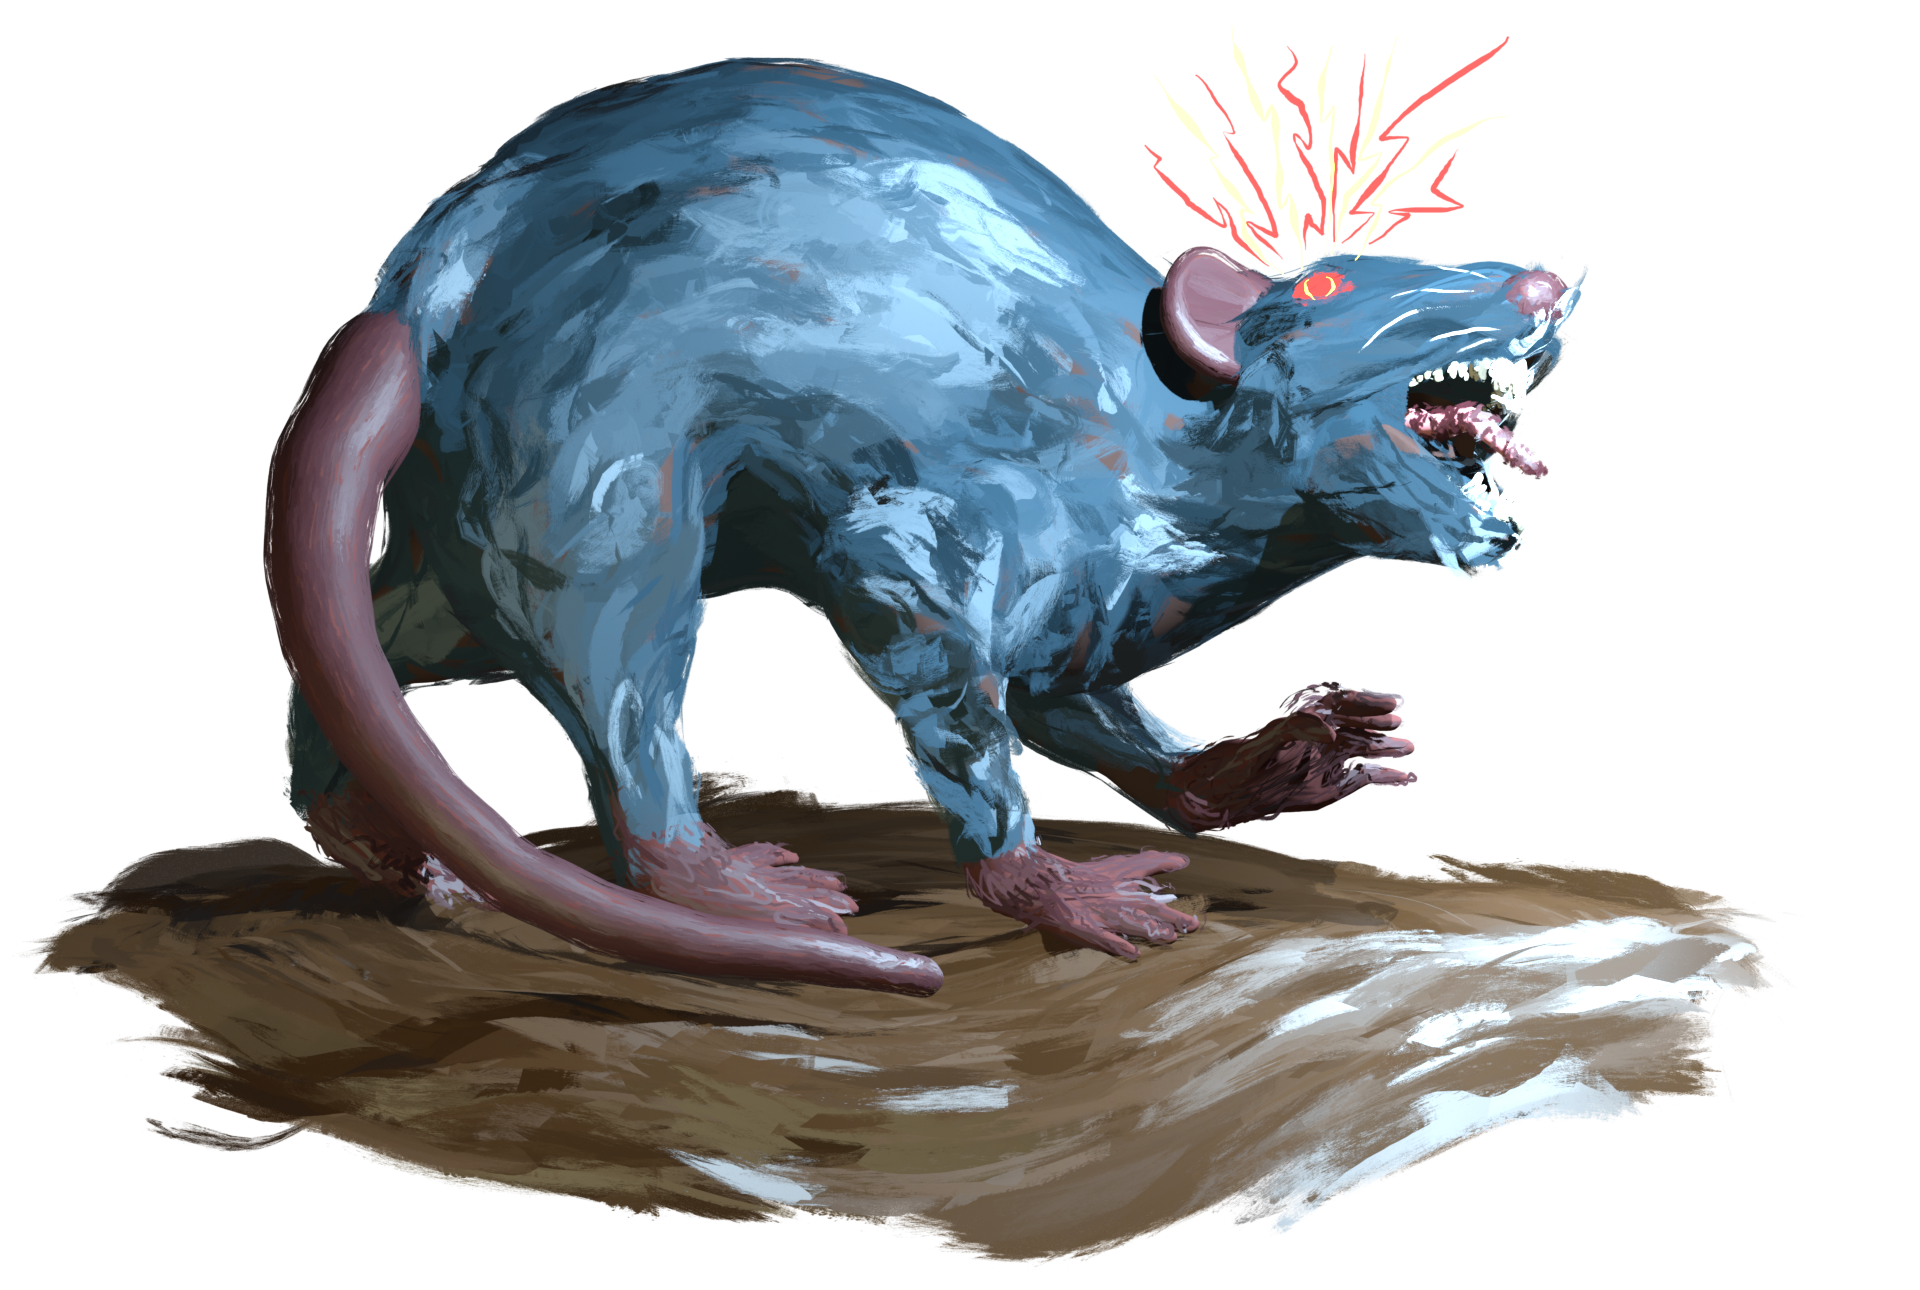
\includegraphics[width=3.2in]{book/img/Giant_Rat}
  \end{minipage}

  Double the amount of rats for the amount of heroes, and the rival group of monster hunters will join in the fight. This is a low-level threat to hook the players immediately into the context. The elder dives out of the way and when the heroes have cleared the rats with the help of their rivals, the elder will return and exhort them to go down into the well and find the source of the blight on their village.
  
  The heroes can press the elder for another possible way into the well and she may explain that there could be another entrance through a cave by the water. Otherwise, they can go down the well itself.
  
  The rival group says they will have better luck up stream in the foothills, and take off to the North.
  
  \subsection{The Caverns}

  \begin{pf-parchment}[\textcolor{title1}{Description}]
    \textcolor{title1}{\textit{The caverns beneath the goblin town are spacious and filled with gigantic, incandescent mushrooms which light the darkness. There is an underground river which runs the length of this cavern from North to South. The churning water in the river is a sickly green and brown color which smells distinctly metallic. As the river winds North, the passage bends to the East and out of sight.}}
  \end{pf-parchment}

  Once down into the caverns beneath the village, the heroes will notice that the water looks poisoned. If the heroes get into the water, they must make Fortitude saves against Scarlet Fever DC 13 Fortitude, gaining sicked 1 on a failure. If they cross the water to the East, they can find a treasure chest which is trapped. The chest is backed up against an old looking, rotted, wooden wall. If the heroes go around the wall through a side passage, they will see that the chest is wired into a trap and can disable the trap from that side. If they do not, and they try to open the chest, they will trigger a Poisoned Lock.

  When they continue North through the cavern they will be confronted with more traps laid by the corrupted Swarm Voice ahead. There are four bear traps on the sides of the cavern which are wide enough to stand on. The heroes can either disarm two of these four traps to go further into the cavern, or they can get into the poisoned water and wade through the center. If the heroes get into the water, they must make Fortitude saves against Scarlet Fever DC 13 Fortitude, gaining sickened 1 on a failure.

  \subsection{The Corrupted Swarm Voice}

  \begin{pf-parchment}[\textcolor{title1}{Description}]
    \textcolor{title1}{\textit{This cavern is wide and opens to a pool which is surrounded by Ratfolk with gleaming red eyes. Red magic energetically sparks from their eyes as they raise their weapons. In the center of this pool is a large rock which crests outside of the sickly looking water.}}
  \end{pf-parchment}

  Once they round the bend they will be greeted by a Corrupted Swarm Voice, who has deployed two more traps in this room, on the North and South sides which lead to him. The Voice has two Tunnel Vipers in this cavern as well.

  When the fight begins, the rival group of monster hunters will emerge from the tunnel to the North and claim the battle to be theirs. As they move in, they will need to disarm the trap to the North and continue their way to the Voice.
  
  During the course of the battle, the Voice will make a corrupting call against the rival group and each one of them will succumb to the call. Their eyes will start glowing red with crackling crackling from it like the Voice's. With an action, they will shake it off one by one, and their eyes will return to normal.
  
  When they defeat the Voice and his Vipers, the heroes and their rivals will discover that the Voice has been poisoning the well with the source here: a corrupted crystal that glows with red energy. Before the rival group can take the crystal from the heroes, they will begin fits of coughing fits with their eyes beginning to glow red once more. Before there is a chance to react, the rivals will run out of the cavern back the way they came from the North.

  \begin{minipage}[t]{.15\textwidth}
    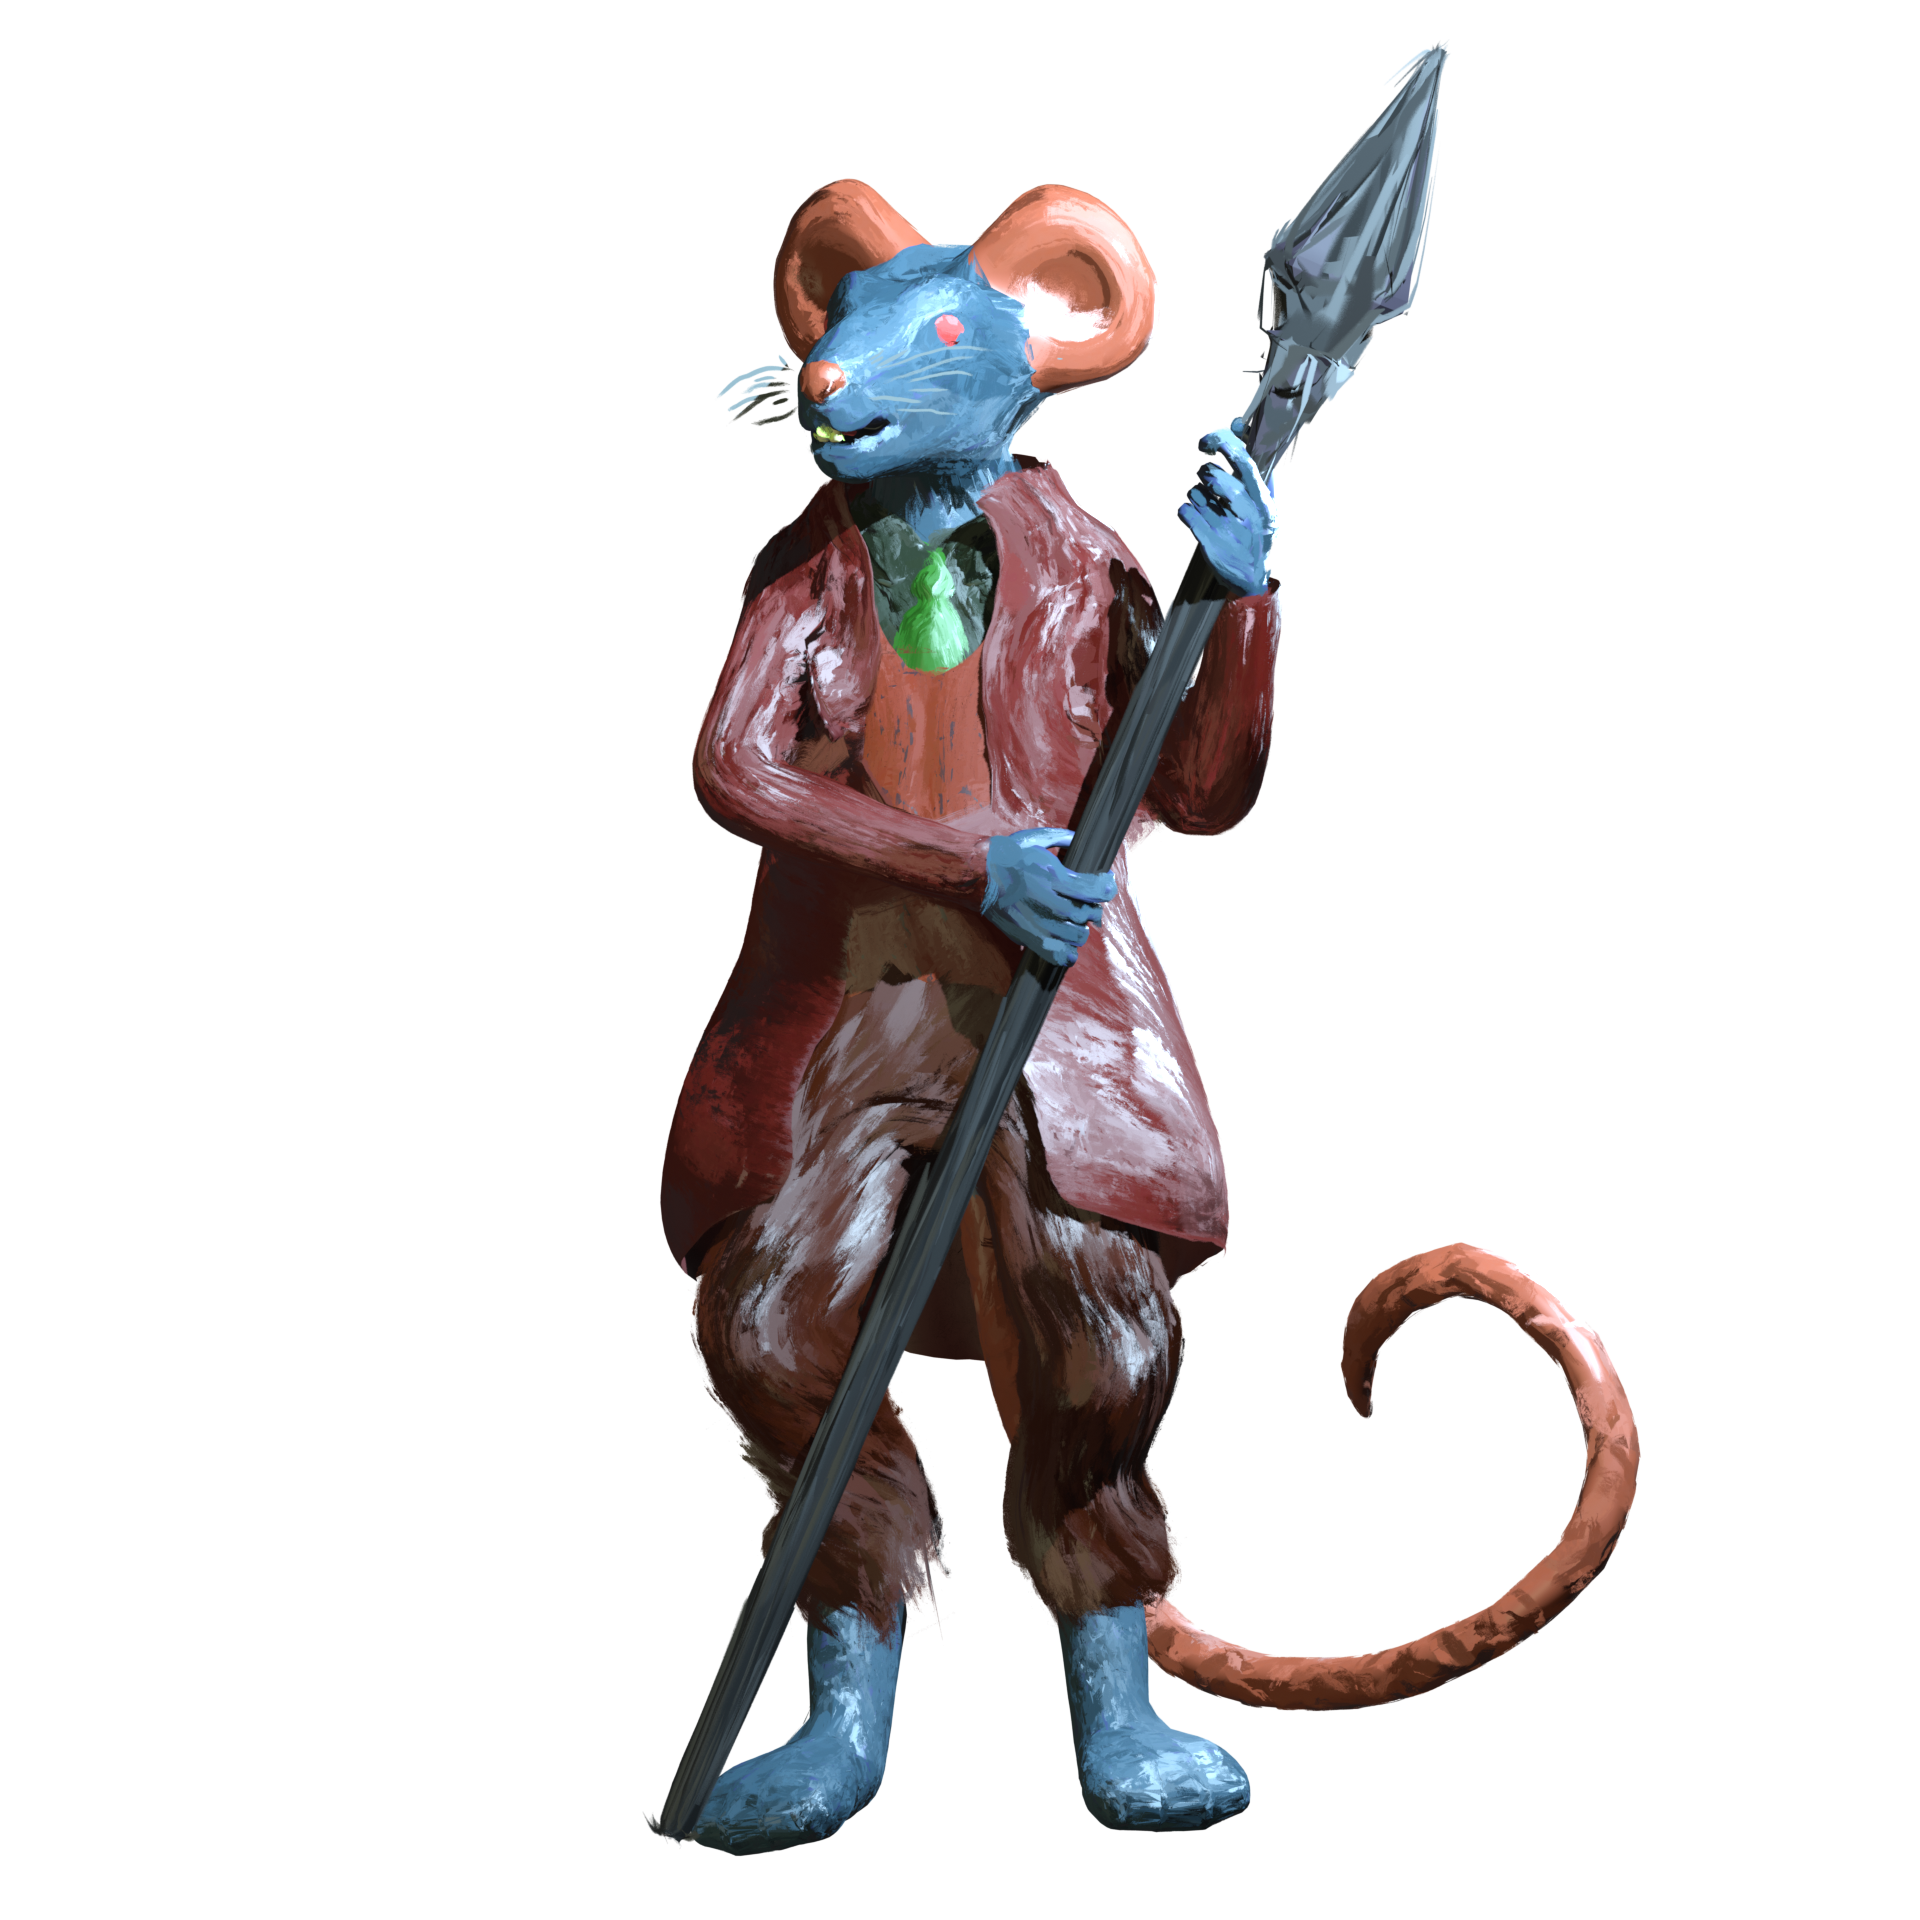
\includegraphics[width=3in]{book/img/Swarm_Voice}
  \end{minipage}

  \section{Conclusion}
  The heroes go back to town to report to the elder that the source of the poison is dealt with. The elder compensates them with 10 gold pieces for their service.

  They don't see any sign of the rival group or their ship when they row back to their own ship. Sarlohmon, their aged wizard who is depleted after attempting to force the reality tear shut, is intrigued by the stone they have uncovered from this corruption. The stone itself is a part of a key of immense power which can summon the closest corrupted being. The crystal appears to have two more pieces before it is whole. He implores the adventurers to keep searching.

\end{multicols}
\pfBigArt{t}{images/altar_bright}